\chapter{Estado del arte y contexto tecnológico}
\label{chap:estado-arte}

\lettrine{E}{ste} capítulo pretende situar el trabajo de fin de grado en el contexto de las tecnologías y enfoques existentes en el ámbito de los sistemas IoT con soporte móvil.

% SUGERENCIA DE REDACCIÓN:
% Aquí encaja un párrafo breve que enmarque el capítulo 2 como revisión de
% arquitecturas, plataformas de captura y métodos de procesado, no solo como
% descripción de dispositivos. La idea sería dejar claro desde el principio que
% el TFG se centra en una arquitectura de adquisición/procesado y que el caso
% de uso marino es el contexto de aplicación.
% Referencias útiles para apoyar ese arranque:
% - A Survey on IoT Application Architectures:
%   https://www.mdpi.com/1424-8220/24/16/5320
% - An Open-Source Smart Sensor Architecture for Edge Computing in IoT Applications:
%   https://www.mdpi.com/373124

Para hablar de IoT es preciso hacer una revisión de las arquitecturas de aplicaciones IoT, centrándose en dónde se capturan, procesan, almacenan y gestionan los datos dentro de un sistema. En este sentido, existe una idea principal: no existe una arquitectura única que sea válida para todos los casos de uso. Cada contexto requiere una solución capaz de equilibrar necesidades distintas, como la latencia, la escalabilidad, el consumo o la privacidad.

Existen tres grandes enfoques:
\begin{itemize}
  \item Cloud, que se centra en la captura de datos en el borde y su procesamiento en la nube, lo que permite una gran capacidad de procesamiento y almacenamiento, pero puede introducir latencia y dependencia de la conectividad.
  \item Edge, que se centra en el procesamiento de datos en el borde, cerca de la fuente de datos, lo que reduce la latencia y la dependencia de la conectividad, pero puede limitar la capacidad de procesamiento y almacenamiento.
  \item Fog, que se centra en el procesamiento de datos en la nube, pero con una capa intermedia de procesamiento en el borde, lo que permite un equilibrio entre la latencia y la capacidad de procesamiento.
\end{itemize}

Cada una de estas arquitecturas tiene ventajas e inconvenientes que, a la hora de diseñar un sistema IoT, deben tenerse en cuenta según las necesidades concretas de la aplicación.

% GUÍA DE REFERENCIAS PARA ESTA PARTE DEL CAPÍTULO:
% - Arquitectura IoT / sistema ciberfísico:
%   https://www.mdpi.com/1424-8220/24/16/5320
%   https://www.mdpi.com/373124
% - Sensado móvil / sensores inerciales de smartphone:
%   https://www.mdpi.com/1424-8220/16/4/477
%   https://doi.org/10.3390/s21237946
% - Nodo embebido / monitorización inalámbrica:
%   https://www.mdpi.com/2076-3417/15/15/8394
%   https://www.mdpi.com/1424-8220/22/22/8937
% - Marco de oleaje y parámetros espectrales:
%   https://www.ndbc.noaa.gov/faq/wavecalc.shtml
%   https://www.ndbc.noaa.gov/faq/wavespectra.shtml
% - Caso aplicado cercano al dominio:
%   https://www.mdpi.com/2076-3263/12/3/110


\section{Caracterización del oleaje mediante parámetros estadísticos}

Una vez introducido el contexto arquitectónico general, resulta necesario describir el dominio de aplicación concreto considerado en este trabajo: la caracterización del oleaje.

Los parámetros estadísticos sirven para describir el estado del mar de una forma general pero útil. El oleaje es un fenómeno complejo y no resulta sencillo caracterizarlo con una sola medida instantánea. De acuerdo con la documentación técnica del National Data Buoy Center (NDBC), una forma habitual de describirlo consiste en emplear parámetros derivados del espectro de energía de la señal. Para este trabajo, los más relevantes son los siguientes:

\begin{itemize}
  \item \textbf{Altura significativa (Hs)}: se aproxima como la altura media del tercio más alto de las olas. En formulación espectral puede expresarse como:
$$ Hs = 4 \sqrt{m_0} $$
donde $m_0$ es el momento espectral de orden cero, que se obtiene integrando la densidad espectral de energía del oleaje:
$$ m_0 = \int_0^\infty S(f) df $$
  \item \textbf{Periodo medio de cruce por cero (Tz)}: en análisis espectral, esta magnitud suele aproximarse mediante los momentos espectrales como:
$$ Tz = \sqrt{\frac{m_0}{m_2}} $$
donde $m_2$ es el momento espectral de orden dos. Este parámetro resume una escala temporal media del oleaje y resulta útil para comparar estados de mar sin necesidad de reconstruir cada ola individual.
  \item \textbf{Periodo pico (Tp)}: se define como el periodo asociado a la frecuencia de máxima energía del espectro, y se calcula como:
$$ Tp = \frac{1}{f_p} $$
donde $f_p$ es la frecuencia con mayor densidad espectral.
\end{itemize} 

El uso de estos parámetros refuerza una idea importante para este TFG: el objetivo no es reconstruir con precisión la forma instantánea de cada ola, sino obtener una caracterización estadística y espectral del estado del mar a partir de señales inerciales. Por ello, el análisis del problema se apoya en magnitudes agregadas como $Hs$, $Tz$ y $Tp$, que son habituales en la instrumentación oceanográfica y encajan de forma natural con un pipeline de procesado basado en espectros.

\begin{figure}[htbp]
  \centering
  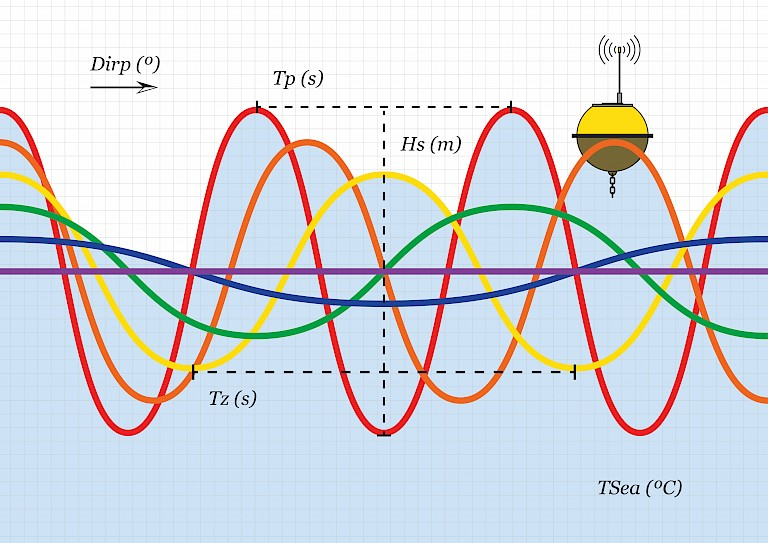
\includegraphics[width=0.82\textwidth]{imaxes/oleaje_parametros.jpg}
  \caption{Representación visual de algunos parámetros característicos del oleaje, como $Hs$, $Tp$ y $Tz$. Fuente: Folkestone Fringe.}
  \label{fig:oleaje-parametros}
\end{figure}

% SUGERENCIA DE REDACCIÓN:
% Aquí quedaría muy bien explicar que en oleaje el objetivo habitual no es la
% altura instantánea de una sola ola, sino parámetros estadísticos y espectrales
% del estado del mar. Conviene nombrar explícitamente Hs, Tz y Tp y enlazarlos
% con el análisis espectral.
% Referencias útiles:
% - NDBC wavecalc:
%   https://www.ndbc.noaa.gov/faq/wavecalc.shtml
% - NDBC wavespectra:
%   https://www.ndbc.noaa.gov/faq/wavespectra.shtml
% - OpenMetBuoy (como ejemplo aplicado con IMU):
%   https://www.mdpi.com/2076-3263/12/3/110


\section{Android como plataforma de sensado de bajo coste}

El desarrollo de IOT tiene un amplio espectro de enfoques y variedad de desarrollos, desde soluciones de hardware dedicado , desarrollo de menos especializado y de codigo abierto, hasta soluciones comerciales cerradas. En este contexto, el uso de smartphones como plataforma de iot es una respuesta inteligente ya que si analizamos las características de los smartphones modernos, vemos que cuentan con una amplia variedad de sensores integrados, incluyendo acelerómetros, giroscopios y magnetómetros, que pueden ser utilizados para capturar datos inerciales sin necesidad de hardware adicional. Además, los smartphones ofrecen capacidades de procesamiento y conectividad que permiten no solo la captura de datos, sino también su procesamiento local y transmisión a servidores o nubes para análisis posterior.\smallskip

Esto permite validar sistemas funcionales sin depender desde el primer momento de hardware específico, y esta reutilización de una plataforma de consumo encaja bien en arquitecturas IoT, en las que un mismo nodo puede asumir varias funciones de forma simultánea: adquisición, preprocesado, visualización y comunicación, especialmente en arquitecturas de tipo edge.

Android aporta además de una base práctica para captura de medidas inerciales una plataforma que ayuda a acelerar la validación del sistema completo, ya que permite ahorrar tiempo de desarrollo en fases tempranas.


Frente a soluciones IoT dedicadas, Android permite iterar rápido y desplegar prototipos funcionales sin depender de hardware específico desde el primer día.\medskip

\begin{figure}[htbp]
  \centering
  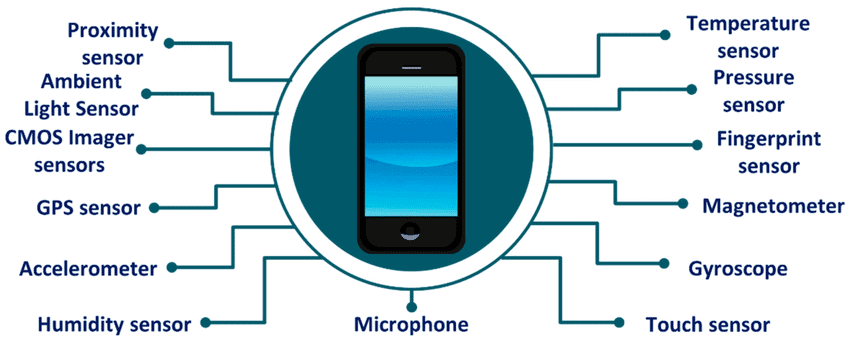
\includegraphics[width=0.8\textwidth]{imaxes/smartphone_sensor_diagram.png}
  \caption{Referencia visual del smartphone como dispositivo de sensado, con integración de sensores y procesamiento local. Fuente: Medium.}
  \label{fig:smartphone-sensado}
\end{figure}

% SUGERENCIA DE REDACCIÓN:
% En este punto encaja un párrafo que sitúe al smartphone como plataforma de
% prototipado y adquisición de bajo coste dentro del estado del arte. La idea
% sería explicar que integra sensores, interfaz, almacenamiento y conectividad,
% lo que acelera la validación temprana del sistema completo.
% Referencias útiles:
% - Evaluation of Smartphone Inertial Sensor Performance for Cross-Platform Mobile Applications:
%   https://www.mdpi.com/1424-8220/16/4/477
% - Experimental Evaluation of Smartphone Accelerometer and Low-Cost Dual Frequency GNSS Sensors for Deformation Monitoring:
%   https://doi.org/10.3390/s21237946


% SUGERENCIA DE REDACCIÓN:
% Si quieres reforzar esta parte, aquí podrías convertir estas ventajas en un
% pequeño párrafo comparativo con soluciones dedicadas: menor coste de entrada,
% menor tiempo de iteración y capacidad de operar/capturar/revisar en el mismo
% dispositivo.
% Referencia útil:
% - Evaluation of Smartphone Inertial Sensor Performance for Cross-Platform Mobile Applications:
%   https://www.mdpi.com/1424-8220/16/4/477


\subsection{Límites de una solución móvil pura}

El enfoque móvil evidentemente presenta claras limitaciones como pueden ser: 
\begin{itemize}
  \item \textbf{Variabilidad entre dispositivos}: Existen innumerables modelos de smartphones en el mercado, cada uno con diferentes sensores, calibraciones y procesamiento; además de esto, existen diferentes versiones de Android, e incluso no tiene por qué ser Android. Teniendo esto en cuenta, no podemos esperar un comportamiento estándar, especialmente si se espera un nivel de precisión mínimamente profesional, por lo que es importante considerar esta variabilidad en el diseño del sistema y en la interpretación de los datos capturados. 
  \item \textbf{Control limitado del hardware sensorial}: Los smartphones no están pensados para ser configurables a nivel de hardware, lo que implica que, aun teniendo acceso, en nuestro caso, a los sensores inerciales, no podemos controlar ciertas características como la frecuencia de muestreo, la sensibilidad, etc. Evidentemente, si comparamos esto con una solución de hardware dedicado, es una desventaja clara. 
\end{itemize}

Si analizamos el rendimiento de los sensores inerciales entre dos smartphones, se aprecian diferencias por varias razones:
\begin{itemize}
  \item \textbf{Diferente hardware físico}: Dos móviles pueden montar sensores MEMS distintos, ya sea por fabricantes, modelos o generaciones, lo que puede resultar en diferencias significativas en la calidad de la señal capturada.
  \item \textbf{Diferente sesgo (bias)}: Aun con el mismo modelo de sensor, cada unidad puede tener un sesgo diferente, ya que se trata de un error sistemático. En el caso de un móvil que está quieto, el acelerómetro debería registrar una aceleración de 0 m/s² en los ejes horizontales y 9.81 m/s² en el eje vertical (debido a la gravedad). Pero cuando lo ponemos en práctica, debido a imperfecciones, puede dar un pequeño desplazamiento constante.
  \item \textbf{Diferente ruido (noise)}: Además de ese desplazamiento constante, aun estando quietos, la señal no es perfectamente estable, sino que presenta pequeñas fluctuaciones aleatorias, y esta oscilación puede ser mayor o menor dependiendo del modelo de móvil, del estado de los sensores, etc.
  \item \textbf{Diferente tratamiento por el sistema operativo}: La app no accede al sensor físico directamente, sino a través del sistema operativo que muchas veces entrega la señal ya procesada, con filtros, ajustes, remuestreos o tratamientos de drivers y capas internas .
  \item \textbf{Diferente frecuencia real de muestreo}: Se puede pedir una frecuencia concreta, pero no siempre se cumple exactamente; puede tener jitter y variar según el modelo o la carga del sistema.
  \item \textbf{Diferente calibración}: Un teléfono puede venir con mejor calibración de fábrica que otro, lo que afecta a la exactitud, linealidad y estabilidad de la señal capturada.
\end{itemize}

% SUGERENCIA DE REDACCIÓN:
% Aquí encaja bien un cierre de la subsección explicando que las limitaciones del
% móvil (variabilidad, autonomía, resistencia, control temporal) justifican una
% arquitectura extensible y no una solución móvil pura.
% Referencias útiles:
% - Evaluation of Smartphone Inertial Sensor Performance for Cross-Platform Mobile Applications:
%   https://www.mdpi.com/1424-8220/16/4/477
% - A Survey on IoT Application Architectures:
%   https://www.mdpi.com/1424-8220/24/16/5320


% SUGERENCIA DE REDACCIÓN:
% Aquí sería muy bueno mencionar explícitamente jitter, frecuencia efectiva de
% muestreo y variabilidad entre dispositivos como limitaciones metodológicas del
% sensado móvil, no solo limitaciones de hardware.
% Referencias útiles:
% - Evaluation of Smartphone Inertial Sensor Performance for Cross-Platform Mobile Applications:
%   https://www.mdpi.com/1424-8220/16/4/477
% - Experimental Evaluation of Smartphone Accelerometer and Low-Cost Dual Frequency GNSS Sensors for Deformation Monitoring:
%   https://doi.org/10.3390/s21237946


\section{Nodos embebidos para adquisición dedicada}
Hay dos razones principales por las que se opta por un nodo embebido además de la solución móvil:
\begin{itemize}
  \item \textbf{Comparación directa de captura}. La idea de usar nodos embebidos es obtener una comparación directa entre la captura que se obtiene con el dispositivo móvil y la captura que se obtiene con el nodo embebido. De esta forma se dispone de un punto de referencia para evaluar la calidad de la propuesta frente a una solución de hardware dedicado, que conllevaría un coste, complejidad y tiempo de desarrollo mayores.
  \item \textbf{Caso de uso extra}. Además de esto, disponer de más de un nodo de captura de datos abre la posibilidad de aplicar otras configuraciones. En este caso, el uso principal es la caracterización de oleaje en un punto concreto, pero si se tienen dos nodos podrían, por ejemplo, colocarse en dos puntos de un barco y obtener datos de ambos lugares para realizar algún tipo de análisis adicional.
\end{itemize}


En este trabajo, esa línea se representa con ESP32+IMU, usando el ESP32 como nodo de captura/comunicación y Android como interfaz de operación. La comparación entre móvil y embebido no se entiende como una sustitución directa, sino como un análisis de compromisos entre simplicidad operativa, control técnico y mantenibilidad.

\begin{figure}[htbp]
  \centering
  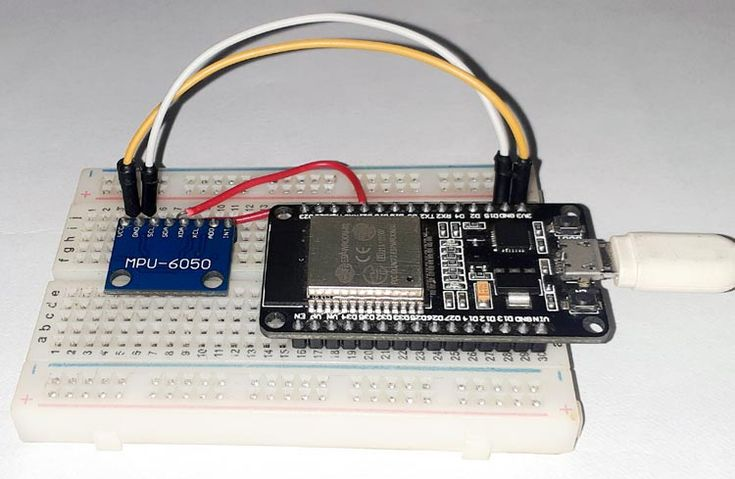
\includegraphics[width=0.62\textwidth]{imaxes/nodo_embebido_conceptual.jpg}
  \caption{Referencia visual del subsistema embebido de captura, formado por una placa de control/comunicación y una IMU externa. Fuente: Pinterest.}
  \label{fig:nodo-embebido-conceptual}
\end{figure}

% SUGERENCIA DE REDACCIÓN:
% Aquí conviene introducir el valor de los nodos embebidos como dispositivos de
% adquisición dedicada: mayor control temporal, control del sensor, buses y
% comunicaciones, además de separación entre captura y explotación.
% Referencias útiles:
% - Microcontroller Unit-Based Wireless Sensor Network Nodes: A Review:
%   https://www.mdpi.com/1424-8220/22/22/8937
% - Design and Validation of the MANTiS-32 Wireless Monitoring System for Real-Time Performance-Based Structural Assessment:
%   https://www.mdpi.com/2076-3417/15/15/8394


% MAPA DE CITAS DENTRO DEL CAPÍTULO:
% - Caracterización del oleaje: NDBC wavecalc + NDBC wavespectra.
% - Android como plataforma: smartphone inertial sensor performance.
% - Límites de la solución móvil pura: smartphone performance + validación experimental.
% - Nodos embebidos: MCU-based WSN nodes review + MANTiS-32.
% - Marco comercial y soluciones profesionales de referencia: Datawell + VectorNav/Xsens.
% - Posicionamiento del trabajo: usar una o dos referencias del dominio solo como contexto, sin dejar que dominen el capítulo.


\section{Marco comercial y soluciones profesionales de referencia}

Para situar adecuadamente la propuesta desarrollada en este TFG, conviene tener en cuenta que el mercado ya dispone de soluciones profesionales específicamente orientadas a la medida de oleaje y al sensado inercial de altas prestaciones. Estas soluciones no constituyen el objetivo directo del trabajo, pero sí ofrecen un marco de referencia útil para entender qué prestaciones, garantías y compromisos son habituales en el ámbito comercial.

En el caso de la medida de oleaje, existen boyas profesionales diseñadas específicamente para operación marina continuada, como las familias Waverider de Datawell. Este tipo de sistemas se orienta a la obtención fiable de parámetros estándar de oleaje, datos espectrales y operación prolongada en condiciones ambientales exigentes. Su interés dentro del estado del arte no reside únicamente en la precisión instrumental, sino también en el hecho de representar una solución consolidada, robusta y pensada desde el inicio para el entorno marino.

De forma complementaria, en el ámbito del sensado inercial existen IMUs industriales y profesionales concebidas para integración técnica en sistemas embebidos y de navegación, como ocurre con soluciones de fabricantes como VectorNav o Xsens. Frente a un smartphone, este tipo de sensores suele ofrecer especificaciones más estables, mejor caracterización de sesgo y ruido, interfaces de integración más controladas y una mayor trazabilidad de las prestaciones declaradas por el fabricante. Esto los convierte en una referencia natural cuando se quiere comparar una solución accesible y flexible con instrumentación específicamente diseñada para tareas de medida o navegación.

Desde esta perspectiva, la propuesta del TFG no pretende competir directamente con una boya oceanográfica profesional ni sustituir una IMU industrial de altas prestaciones. Su interés se sitúa en otro plano: explorar una arquitectura de adquisición y procesado de bajo coste, flexible y extensible, capaz de integrar plataformas heterogéneas y de comparar distintos compromisos entre accesibilidad, control técnico y complejidad de despliegue.

\begin{figure}[htbp]
  \centering
  \begin{minipage}[t]{0.58\textwidth}
    \centering
    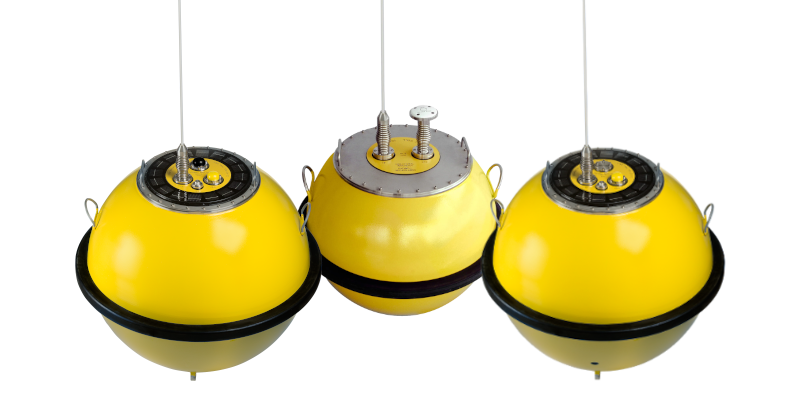
\includegraphics[width=\textwidth]{imaxes/datawell_buoys.png}
  \end{minipage}\hfill
  \begin{minipage}[t]{0.34\textwidth}
    \centering
    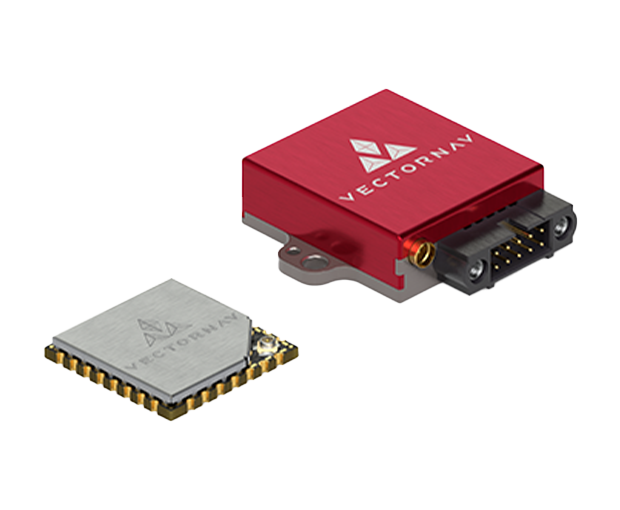
\includegraphics[width=\textwidth]{imaxes/vectornav_vn200.png}
  \end{minipage}
  \caption{Ejemplos de soluciones profesionales de referencia en medida de oleaje y sensado inercial: familia de boyas Datawell Waverider (izquierda) y sensor VectorNav VN-200 (derecha). Fuentes: Datawell y VectorNav.}
  \label{fig:referencias-profesionales}
\end{figure}

\begin{table}[htbp]
  \centering
  \small
  \begin{tabularx}{\textwidth}{>{\raggedright\arraybackslash}p{0.22\textwidth} >{\raggedright\arraybackslash}X >{\raggedright\arraybackslash}X >{\raggedright\arraybackslash}X}
    \rowcolor{udcpink!25}
    \textbf{Aspecto} & \textbf{Smartphone} & \textbf{Nodo embebido propio} & \textbf{Solución profesional} \\
    Coste de entrada & Muy bajo, al reutilizar hardware de consumo & Moderado, con necesidad de integración y montaje & Alto, por tratarse de instrumentación específica \\
    Control del sensor & Limitado por hardware y sistema operativo & Alto, al poder elegir interfaz, bus y configuración & Alto, con especificaciones y calibración declaradas \\
    Robustez instrumental & Variable entre dispositivos & Dependiente del diseño e integración realizada & Alta, pensada para operación prolongada \\
    Tiempo de despliegue & Muy rápido & Medio, requiere integración hardware/software & Bajo una vez adquirido, pero con mayor barrera de acceso \\
    Flexibilidad arquitectónica & Alta para prototipado y validación inicial & Alta, con mayor control técnico & Más limitada al producto adquirido \\
    Objetivo principal & Accesibilidad y validación rápida & Adquisición dedicada y comparación técnica & Medida fiable y operación profesional \\
  \end{tabularx}
  \caption{Comparación general entre smartphone, nodo embebido propio y soluciones profesionales de referencia.}
  \label{tab:comparativa-marco-comercial}
\end{table}

% SUGERENCIA DE REDACCIÓN:
% Si quieres reforzar esta sección, aquí puedes citar una boya profesional como
% referencia instrumental consolidada y una o dos IMUs industriales como ejemplo
% de sensado inercial de mayor control y especificación.
% Referencias útiles:
% - Datawell:
%   https://datawell.nl/
%   https://datawell.nl/products/wave-unit/
% - VectorNav VN-200:
%   https://www.vectornav.com/products/detail/vn-200
% - Xsens MTi-1:
%   https://www.movella.com/products/sensor-modules/xsens-mti-1-imu


\section{Posicionamiento del trabajo}

La aportación del TFG se sitúa en la integración de arquitectura, no en un único componente aislado.
El trabajo se posiciona como una propuesta de sistema ciberfísico modular que cubre adquisición, comunicación, persistencia y operación.

\begin{table}[htbp]
  \centering
  \small
  \begin{tabularx}{\textwidth}{>{\raggedright\arraybackslash}p{0.24\textwidth} >{\raggedright\arraybackslash}X >{\raggedright\arraybackslash}X}
    \rowcolor{udcpink!25}
    \textbf{Aspecto} & \textbf{Enfoques frecuentes} & \textbf{Enfoque del TFG} \\
    Plataforma base & App móvil o nodo embebido por separado & Arquitectura híbrida Android+ESP32 \\
    Persistencia & Almacenamiento local o backend ad-hoc & Persistencia desacoplada con alternativas evaluables \\
    Integración & Piezas aisladas (captura, visualización, etc.) & Flujo extremo a extremo con contratos comunes \\
    Evolución técnica & Cambios con alto acoplamiento & Diseño modular con sustitución de capas \\
  \end{tabularx}
  \caption{Posicionamiento resumido del trabajo frente a enfoques habituales.}
  \label{tab:estado-arte-posicionamiento}
\end{table}

% SUGERENCIA DE REDACCIÓN:
% El cierre puede insistir en que la aportación principal no es una boya ni una
% app aislada, sino una arquitectura comparativa con dos plataformas de captura
% y un pipeline común de explotación.
% Referencias útiles para apoyar ese cierre:
% - A Survey on IoT Application Architectures:
%   https://www.mdpi.com/1424-8220/24/16/5320
% - OpenMetBuoy (solo como referencia aplicada de contexto):
%   https://www.mdpi.com/2076-3263/12/3/110
